For storage of acquired data a centralized server has been implemented. Storing
all acquired experimental data in a database on a centralized server running
open source software has a number of attractive features. Firstly, by storing
the data on a centralized server, backup of all experimental data is enormously
simplified compared to backup of individual computers. Backup of experimental
data on the local client is hence, from a user's point of view, transparent as
this can be performed by routine jobs on the server. Secondly, the data is
stored in a standardized and open format which allows easy export of the data
to any platform, open format or software source making data exchange across
different platforms simpler. Thirdly, by open sourcing all of the code
collaboration between several different groups is possible thus increasing the
number of developers to optimize the code and further increase functionality.

A centralized storage of data can be accomplished in many ways. However, in
experimental laboratories where large amounts of data are recorded a database
is an obvious choice for storage. To keep the server backed simple we are using
a relational database. As specific implementation we have chosen MySQL due to
its GNU General Public License, simplicity, fast performance, flexibility and
scalability.

A system design of many highly decentralized clients all pushing data
continuously to a central MySQL server requires high server performance, high
uptimes as well as a flexible storage ensuring easy expansion of storage space
if needed. To ensure these properties of the system it has been designed as
simple as possible to avoid unnecessary complications and to ensure that this
central component can be easily managed by the professional IT-staff at the
department. It is important to realize that even though it is typically not a
problem if a single client machine somewhere in the system is temporarily down
(this can happen for many reasons in a experimental lab) it is crucial that the
server is handled like a real production server.

To protect against pollution of the various setups tables in the database each
client has its own username and password which is not part of the code
(typically it will be managed in the local ODBC-settings of the client). In
this way, interface code can flow back and forth between different setups
without the risk of one setup accidentally logging data to other setup's
tables.

\subsection{Data extraction} 
The flexible nature of SQL allows one to extract data in many
ways. Complete datasets can be retrieved by simple statements 

\begin{verbatim}
 select {*} from table_name
\end{verbatim}

This data can the be handled using the programming environment most comfortable
for users and can be used to perform automatic reporting, data treatment or as
input to scripts that will produce plots based on the data. SQL also allows for
very efficient data treatment directly from the SQL-server which can be very
useful to get a quick overview of the acquired data. As an example SQL
statements can be used to plot the pressure in a vacuum chamber at 1\,A.M. in
the morning for the last month. This can be a useful tool to monitor the
general health of the chamber, i.e. if leaks has developed, a valve is
failing, a roughing pump is malfunctioning etc.

\begin{verbatim} 
select unix_timestamp(date(time)), avg(pressure) from
pressure_microreactor where hour(time) = 1 and minute(time) between 00 and 20
and time between {from} and {to} group by date(time) order by time desc limit
30; 
\end{verbatim}
where \{from\}  and \{to\} should be replaced with the
relevant time interval.

The output from as a statement like this is illustrated in
Figure~\ref{fig:morning_pressure}.
\begin{figure}
 \begin{center}
 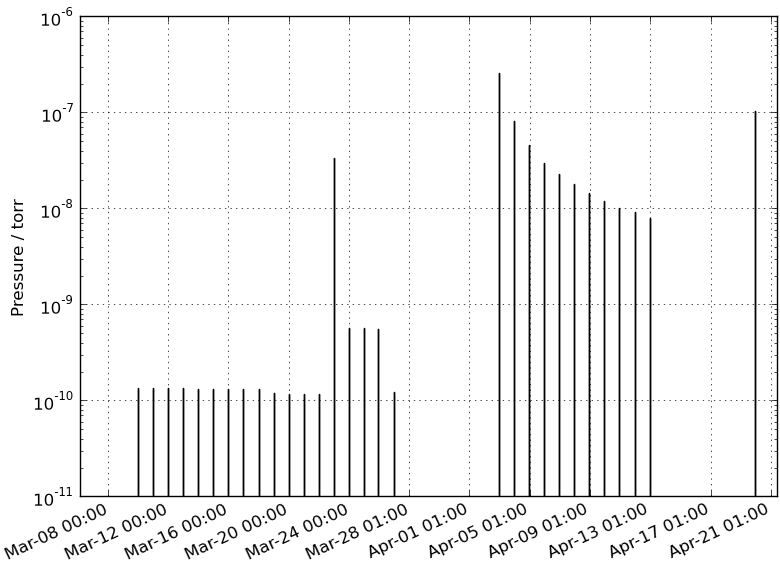
\includegraphics[width=10cm]{morning_pressure.png}
 \caption{ The morning pressure in a vacuum chamber at the department. The
   pressure gauge is unable to read high pressures, and thus no data is
   available from periods where the chamber is vented for maintenance.
   \label{fig:morning_pressure}
 } 
 \end{center}
\end{figure}

A further advantage of SQL servers is the standardization making it easy to
change the choice of implementation if this for some reason is wanted. Several
open source implementations of SQL-servers exists including Firebird,
PostgreSQL, Oracle, Mimer SQL etc..



